\begin{activity}\label{A:0.3.1}
    Consider the function $f(x)$ displayed in Figure \ref{F:0.3.Act1}.
    \ba
        \item Plot $g(x) = -f(x)$ and $h(x) = f(x)-1$.
        \item Define the function $k(x) = -f(x)-1$.  Does it matter which order you
            complete the tranformations from part (a) to result in $k(x)$?  Plot the
            functions resulting from doing the two transformation in part (a) in opposite
            orders.  Which of these functions is $k(x)$?
    \ea
    \begin{figure}[h!]
        \begin{center}
%             \begin{tikzpicture}[scale=0.75]
%                 \draw[color=gray] (-3,-3) grid (3,3);
%                 \draw[thick, black, <->] (-3,0) -- (3,0) node[anchor=west]{$x$};
%                 \draw[thick, black, <->] (0,-3) -- (0,3) node[anchor=west]{$y$};
%                 \draw[very thick, blue] (-2,1) -- (-1,-2) -- (0,-2) -- (1,1) -- (2,-1)
%                 node[anchor=north]{$f(x)$}; 
%             \end{tikzpicture}
%             \begin{tikzpicture}[scale=0.75]
%                 \draw[color=gray] (-3,-3) grid (3,3);
%                 \draw[thick, black, <->] (-3,0) -- (3,0) node[anchor=west]{$x$};
%                 \draw[thick, black, <->] (0,-3) -- (0,3) node[anchor=west]{$y$};
%             \end{tikzpicture}
            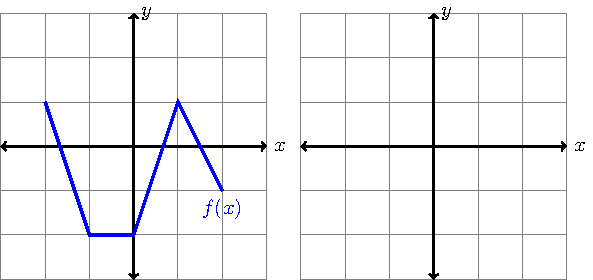
\includegraphics[width=0.65\columnwidth]{figures/0-3-fig2.pdf}
        \end{center}
        \caption{Function transformation for Activity \ref{A:0.3.1}} \label{F:0.3.Act1}
    \end{figure}
\end{activity}
\begin{smallhint}
    \ba
        \item Think of the ``$-$'' in front of $f(x)$ as a $-1$.  What is the difference
            between multiplying by $-1$ and adding $-1$?
        \item Think about the order of mathematical operations.
    \ea
\end{smallhint}
\begin{bighint}
    \ba
        \item $g(x)$ should be a vertical stretch and $h(x)$ should be a vertical shift.
        \item A very methodical way to approach this problem would be to choose several
            particular $x$ values and follow the order of operations to determine the
            output for $k$.
    \ea
\end{bighint}
\begin{activitySolution}
    \ba
        \item The function $g(x)$ should change the sign on all of the $y$ values of $f$.
            The function $h(x)$ will shift all of the $y$ values of $f$ down 1 unit.
        \item The order in which you do the transformations does matter.  In this problem
            the order of operations should be to change the sign on the $y$ value and then
            to shift 1 unit down.
    \ea
    \begin{center}
        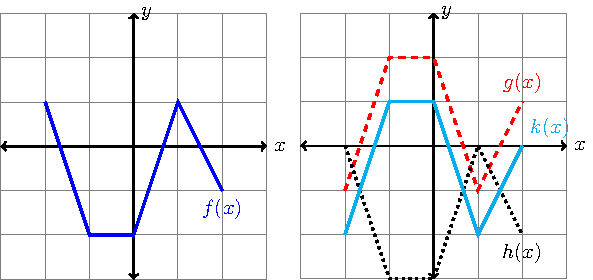
\includegraphics[width=0.65\columnwidth]{figures/0-3-fig2soln.pdf}
    \end{center}
\end{activitySolution}

\aftera
